\documentclass{exam}
\usepackage[utf8]{inputenc}
\usepackage{lmodern}
\usepackage{microtype}

% \usepackage[parfill]{parskip}
\usepackage[dvipsnames]{xcolor}
\usepackage{amsmath}
\usepackage{amsfonts}
\usepackage{amsthm}
\usepackage{siunitx}
\DeclareSIUnit\year{yr}
\DeclareSIUnit\foot{ft}
\DeclareSIUnit\litre{\liter}

\usepackage{skull}

\usepackage{pgfplots}
\usepgfplotslibrary{polar}
\pgfplotsset{compat=1.11}
\usepgfplotslibrary{statistics}
\usepackage{graphicx}
\usepackage{sidecap}
\sidecaptionvpos{figure}{c}
\usepackage{float}
\usepackage{gensymb}
\usepackage{tkz-euclide}
\usetkzobj{all}
\usepackage{commath}
\usepackage{hyperref}
\usepackage{enumitem}
\usepackage{wasysym}
\usepackage{multicol}
\usepackage{mathtools}
\usepackage{tcolorbox}
\usepackage{tabularx}
\usepackage[version=4]{mhchem}
\usepackage{changepage}
\usepackage{listings}
\lstset{basicstyle=\ttfamily\linespread{0.8}\small}

\renewcommand*{\thefootnote}{\fnsymbol{footnote}}

\newtheorem*{thm}{Theorem}
\newtheorem*{iden}{Identity}
\newtheorem*{lemma}{Lemma}
\newtheorem{obs}{Observation}
\theoremstyle{definition}
\newtheorem*{defn}{Definition}
\newtheorem*{ex}{Example}
\newtheorem{con}{Construction}
\newtheorem*{alg}{Algorithm}

\newtheoremstyle{break}
  {\topsep}{\topsep}%
  {\itshape}{}%
  {\bfseries}{}%
  {\newline}{}%
\theoremstyle{break}
\newtheorem*{bthm}{Theorem}

% russian integral
\usepackage{scalerel}
\DeclareMathOperator*{\rint}{\scalerel*{\rotatebox{17}{$\!\int\!$}}{\int}}

% \DeclareMathOperator*{\rint}{\int}

\pgfplotsset{vasymptote/.style={
    before end axis/.append code={
        \draw[densely dashed] ({rel axis cs:0,0} -| {axis cs:#1,0})
        -- ({rel axis cs:0,1} -| {axis cs:#1,0});
    }
}}

% \pointsinrightmargin
\boxedpoints
\pointname{}

\newcommand{\questioA}{\question[\texttt{\textbf{\color{Cerulean} A}}]}
\newcommand{\questioM}{\question[\texttt{\textbf{\color{PineGreen} M}}]}
\newcommand{\questioE}{\question[\texttt{\textbf{\color{WildStrawberry} E}}]}
\newcommand{\questioS}{\question[\texttt{\textbf{\color{Goldenrod} S}}]}
\newcommand{\questioO}{\question[\texttt{\textbf{\color{BurntOrange} O}}]}

\newcommand{\parA}{\part[\texttt{\textbf{\color{Cerulean} A}}]}
\newcommand{\parM}{\part[\texttt{\textbf{\color{PineGreen} M}}]}
\newcommand{\parE}{\part[\texttt{\textbf{\color{WildStrawberry} E}}]}
\newcommand{\parS}{\part[\texttt{\textbf{\color{Goldenrod} S}}]}
\newcommand{\parO}{\part[\texttt{\textbf{\color{BurntOrange} O}}]}

\newcommand{\subparA}{\subpart[\texttt{\textbf{\color{Cerulean} A}}]}
\newcommand{\subparM}{\subpart[\texttt{\textbf{\color{PineGreen} M}}]}
\newcommand{\subparE}{\subpart[\texttt{\textbf{\color{WildStrawberry} E}}]}
\newcommand{\subparS}{\subpart[\texttt{\textbf{\color{Goldenrod} S}}]}
\newcommand{\subparO}{\subpart[\texttt{\textbf{\color{BurntOrange} O}}]}

\newcommand{\mainHeader}[2]{\section*{NCEA Level 2 Mathematics\\#1. #2}}
\newcommand{\mainHeaderHw}[2]{\section*{NCEA Level 2 Mathematics (Homework)\\#1. #2}}
\newcommand{\seealso}[1]{\begin{center}\emph{See also #1.}\end{center}}
\newcommand{\drills}[1]{\begin{center}\emph{Drill problems: #1.}\end{center}}
\newcommand{\basedon}[1]{\begin{center}\emph{Notes largely based on #1.}\end{center}}


\begin{document}

\mainHeaderHw{16}{Counting and Combinatorics}
\subsection*{Reading}
\begin{center}
\begin{tcolorbox}[width=0.8\textwidth,colback={white},title={\textbf{Go and watch...}},colbacktitle=black,coltitle=white]
  \textcolor{black}{\url{https://www.youtube.com/watch?v=aSsCU0mT-Bk}}
\end{tcolorbox}
\end{center}

\begin{center}
\begin{tcolorbox}[width=0.8\textwidth,colback={white},title={\textbf{What's it good for?}},colbacktitle=MidnightBlue,coltitle=white]
  People use combinatorics for...
  \begin{itemize}
    \item Computer science: combinatorics (both the counting we did this week, and the work we'll do over the next few weeks) is a
          foundation of computer science as it allows the efficiency of various algorithms to be measured.
    \item Statistics and probability: if you want to measure probabilities, you need to be able to count how many ways each possibility
          can occur!
    \item Mathematics: combinatorics is one of the fastest-growing areas of modern mathematics, as many modern problems are phrased in
          terms of the discrete (that is, individual pieces and finite sets) rather than the continuous (infinite sets, as studied in calculus).
  \end{itemize}
\end{tcolorbox}
\end{center}

\subsection*{Questions}
\begin{questions}
  \question How many different ways are there to pick seven numbered tennis balls from a bucket of ten, and then order them?
  \question Check that
            \begin{gather*}
              1 = 1\\
              1 + 3 = 4\\
              1 + 3 + 5 = 9\\
              1 + 3 + 5 + 7 = 16\\
              1 + 3 + 5 + 7 + 9 = 25\\
              \cdots
            \end{gather*}
            Generalise (i.e. state and prove some result for all sums of odd numbers). Hint:
            \begin{center}
              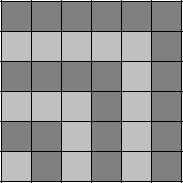
\includegraphics[width=0.3\textwidth]{sumodd}
            \end{center}
  \question The first few powers of 11 are rows of Pascal's triangle (11, 121, 1331, ...). Is this a coincidence? (Hint: no.)
  \question Extension question. If you have $ n $ pieces of spaghetti (each arbitrarily long), and you cross them such that
            every piece crosses every other piece exactly once, how many crossing points are there?
\end{questions}

\end{document}
